\graphicspath{{images/}}

\section{Introduction to Tree-Based Methods}

This group project was focused on the implementation of three different \textbf{tree-based} methods, a collection of statistical learning methods that can be used for regression as well as classification tasks.

At a very high level, these methods divide the predictor space into a number of regions. The prediction for a given observation is then made based upon the mean or mode of the target value for the training data in the region to which it belongs.

The rules that go into segmenting the predictor space can be visualized in the form of a tree structure, because of which these methods are called \textit{tree-based} or \textit{decision-tree} based methods.

In this project, we implemented classifiers based on tree-based algorithms, including \textbf{~\nameref{sec:dt}}, \textbf{~\nameref{sec:rf}}, and \textbf{~\nameref{sec:gb}}.

\subsection{Decision Trees} \label{sec:dt}

Decision Trees \cite{fernandez_decision_tree} are a class of machine learning algorithms capable of performing classification, prediction (regression), as well as multi-output tasks. These are the fundamental building blocks of \textbf{Random Forests} discussed in the following section. The two main kinds of decision trees are \textbf{Regression Trees} and \textbf{Classification Trees}.

\subsubsection{Regression Trees}

When a decision tree is used to predict a numerical value, we refer to it as a Regression Tree. A regression tree is built by the following two steps:

\begin{itemize}
    \item The predictor space is divided into $j$ distinct and non-overlapping regions, $R_{1}, R_{2}, \cdots,R_{j}$
    \item For every observation that falls into region $R_{j}$, we make the same prediction, which is simply the mean of the response values for the training observations in $R_{j}$.
\end{itemize}

We divide the predictor space into high-dimensional boxes, akin to a 2-dimensional rectangle or a 3-dimensional cuboid.

The goal is to find $R = \{R_{1}, R_{2}, \cdots,R_{j}\}$ that minimize the \textbf{Residual Sum of Squares} given by

$$
    \sum_{j=1}^{J} \sum_{i \in R_j} (y_i - \hat{y}_{R_j})^2
$$

where $\hat{y}_{R_j}$ is the mean response for the training observations within the $j^{th}$ box.

However, this approach turns out to be computationally expensive, as considering every possible partition of the feature space into $j$ boxes does not scale very well. This necessitates a \textbf{top-down, greedy} approach called \textbf{recursive binary splitting}.


\subsubsection{Classification Trees}

A classification tree is very similar to a regression tree, except that it is used to predict a categorical variable as opposed to a numeric one. In the case of a regression tree, it was seen that the predicted response for an observation is given by the mean response of the training observations that belong to the same terminal node.
In contrast, a classification tree is used to predict the class of observations that each instance in the testing set belongs to.


In interpreting the results of a classification tree, we are interested not only in the class prediction corresponding to a particular terminal node region, but also in the class proportions among the training observations that fall into that region.

\subsubsection{Advantages and Disadvantages of Decision Trees}
The advantages and disadvantages of using decision trees over other standard methods are enlisted in ~\autoref{tab:dt_adv}.

\begin{table}[H]
    \centering
    \caption{Advantages and Disadvantages of Decision Trees}
    \label{tab:dt_adv}
    \begin{tabularx}{\textwidth}{X|X}
        \hline
        \textbf{Advantages}                                                                                                                                      & \textbf{Disadvantages}                                                                                                                                         \\
        \hline                                                                                                                                                                                                                                                                                                                    \\
        1. \textbf{Easily understood:} The tree structure visualizes the decision-making process, interpretable by both non-technical and technical individuals. & 1. \textbf{Accuracy challenge:} Decision trees exhibit lower accuracy compared to leading supervised learning methods due to high variance and low bias.       \\ \\
        2. \textbf{Handles complex datasets:} Easily manages mixed numerical and categorical predictors without requiring dummy variables.                       & 2. \textbf{Sensitivity to orientation:} Optimal performance relies on orthogonal decision boundaries, favoring linearly separable datasets.                    \\ \\
        3. \textbf{Systematic approach:} Mirror human decision-making process with rule-based methodology.                                                       & 3. \textbf{Variance sensitivity:} Decision trees are highly sensitive to variance, with slight hyperparameter changes leading to significant model variations. \\ \\
        \hline
    \end{tabularx}
\end{table}
\FloatBarrier

\subsection{The Optimization Problem}

As we saw previously, in the case of regression problems, the binary splits in the decision tree growing processes are based on \textbf{minimizing the RSS} values.

In the case of classification problems, the RSS is no longer an effective criterion to make the binary splits in the tree-growing process.
A better alternative is the \textbf{classification error rate}. It is known that an instance in a particular region is going to be assigned to the most commonly occurring label/class of training instances in that region. Therefore, the \textbf{classification error rate} can be defined as the number of training observations in a region that do not belong to the most represented label/class, given by:

$$
    E = 1 - \max_k(\hat{p}_{mk})
$$

where $\hat{p}_{mk}$ refers to the proportion of training instances in the $m^{th}$ region that are from the $k^{th}$ class.

However, these classification errors are not sensitive to the tree-growing process, because of which two other metrics are considered preferable, namely the Gini Index and the Entropy.

\subsubsection{Gini Index}

The \textbf{Gini Index} is given by:

$$
    G = \sum_{k=1}^{K} \hat{p}_{mk} (1 - \hat{p}_{mk})
$$

It is a measure of total variance across the $K$ classes.
The value of this index will be small if all the $\hat{p}_{mk}$ values are close to zero or one,
because of which the Gini Index is considered a measure of node purity.

\textbf{Smaller values of the Gini Index indicate higher purity, signifying that a node contains predominantly observations from one single class}.

\subsubsection{Entropy}

A concept that originates from contemporary information theory, entropy is calculated as:

$$
    D = - \sum_{k=1}^{K} \hat{p}_{mk} \log \hat{p}_{mk}
$$

Considering $\hat{p}_{mk}$ takes a value between 0 and 1, it is safe to say that $ 0 \leq \hat{p}_{mk} \log \hat{p}_{mk}$.

Since the classifiers in this group project are tested against a binary classifier ($K=2$). In the case of such a binary classification, the value of entropy can be further simplified as:

$$
    H(X) = -p \log_2 p - (1 - p) \log_2 (1 - p)
$$

where $p$ refers to P($X = 1$).

Upon plotting H(X) against the probability of class representation, we get this curve:

\begin{figure}[H]
    \centering
    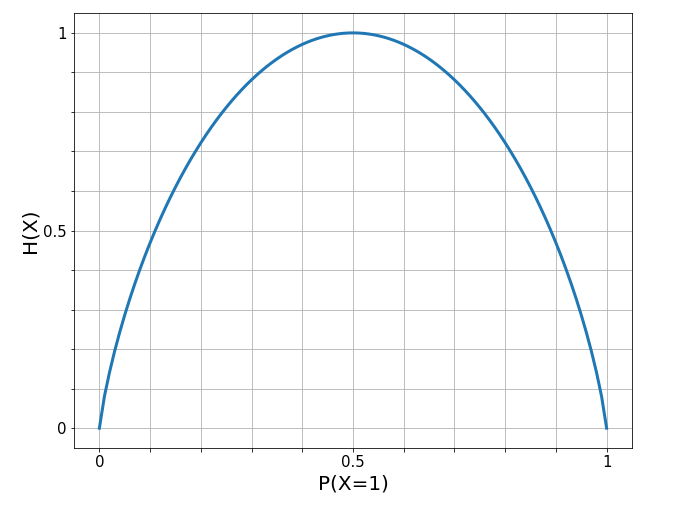
\includegraphics[width=0.65\textwidth]{entropy.png}
    \caption{Entropy vs. Purity}
\end{figure}


Entropy is minimized when all samples in a given node belong to the same class. This can be seen from the fact that the value of entropy will take on a value closer to zero when all the $\hat{p}_{mk}$ values are near zero or one.
That is, the purer the node, lesser the value of entropy.
Conversely, entropy is maximized when there is a uniform class distribution. Surprisingly enough, this definition of entropy clearly seems to align with the literal thermodynamic interpretation of entropy.

\textbf{When splitting a node, it is preferred to minimize the value of entropy so that the node is as pure as possible, and the classification is as certain as possible.}

\subsubsection{Information Gain}

Information gain is defined as a measure of how much information is gained when a node is split at a particular value. In practice, it is the comparison of the entropy values before and after a split.

The specific formula of information gain is given by:

\[
    IG(D) = I(D_p) - \frac{N_{\text{left}}}{N_p}I(D_{\text{left}}) - \frac{N_{\text{right}}}{N_p}I(D_{\text{right}})
\]

where \( D_p, D_{\text{left}}, D_{\text{right}} \) represent the datasets from the parent, left, and right children nodes respectively, \( N_p, N_{\text{left}}, N_{\text{right}} \) represent the number of observations in the parent, left and right children nodes, and \( I(D) \) denotes the entropy for that particular node. At a high level, this formula simply distills down to:

\[
    IG_{A, B} = S_{B} - S_{A}
\]

$S_{B}$ is a measure of how uncertain we were with our data \textbf{before} we made the split, and $S_{A}$ is a measure for how uncertain we are \textbf{after} we split the data. In terms of optimization, we seek to to split a node at a value in a way such that the information gain is maximized.

This optimization problem is a combinatorial optimization problem. The process involved in finding the best decision tree is considered to be a combinatorial problem since it involves selecting the best combination of splits from a given set of finite splits. This optimization problem is also inherently non-convex since there is no smooth function that we need to explicitly maximize or minimize.  Considering the fact the number of potential trees can grow exponentially with the number of features and the depth of the tree, finding an optimal decision tree is an NP-complete problem.

Heuristic methods like greedy algorithms are used to build decision trees, recursively choosing the best split based on a criterion, namely the information gain for classification trees and MSE for regression trees. Each split is chosen to best reduce the impurity of the resulting child nodes, which can be seen as a local optimization problem; however, this greedy approach wouldn't lead to a globally optimal tree.

\textbf{To summarize, in the case of a regression tree, we seek to find the split that minimizes the mean squared error within each node, whereas in the case of classification problems, we seek to choose a split that results in the maximum information gain (or maximum reduction in entropy) to reduce uncertainty in the class labels.}


\subsection{Random Forests} \label{sec:rf}

Random Forest \cite{brownlee2018} \cite{carbonati_rf_scratch} \cite{enoz_rf_medium} is an \textit{ensemble learning} algorithm (one that combines multiple learning algorithms to obtain a better model) that combines the output of many several decision trees (multiple trees = forest!) to get a single result, typically using the process of \textbf{bagging} and \textbf{bootstrapping}.
In order to better understand the concept of Random Forest Models and how they work, it is imperative to understand the concepts of \textbf{~\nameref{app:sec:bootstrapping}} and \textbf{~\nameref{app:sec:bagging}}, which are discussed in the appendix.

In summary, \textbf{Random Forest} models effectively harness the concepts of bagging and bootstrapping creating a bunch of decision trees with an element of randomness baked into them.
This randomness is critical to ensure that constituent individual trees have low correlations with each other, leading to reduced bias.
In addition, the creation of multiple decision trees reduces the risk of overfitting caused by incorporating too much noise from the training dataset.
The mechanics of building a Random Forest are summarized in ~\autoref{fig:rf}.

\begin{figure}[!htbp]
    \centering
    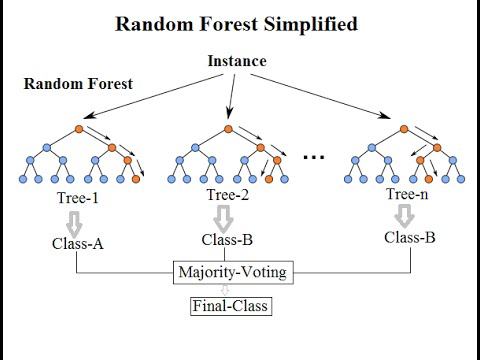
\includegraphics[width=0.65\textwidth]{img-3.png}
    \caption[Random Forests, simplified.]{Random Forests, simplified.\protect \footnotemark}
    \label{fig:rf}
\end{figure}
\footnotetext{Source: \href{https://www.kdnuggets.com/2017/10/random-forests-explained.html}{KDnuggets}}
\FloatBarrier


\subsubsection{Advantages and Disadvantages of Random Forests}
The advantages and disadvantages of using random forests are enlisted in ~\autoref{tab:rf_adv}.
\begin{table}[H]
    \centering
    \caption{Advantages and Disadvantages of Random Forests}
    \label{tab:rf_adv}
    \begin{tabularx}{\textwidth}{X|X}
        \hline
        \textbf{Advantages}                                                                           & \textbf{Disadvantages}                                                           \\
        \hline                                                                                                                                                                           \\
        1. Performs well for both regression and classification.                                      & 1. Accuracy outperforms decision trees but lags behind boosted ensemble methods. \\ \\
        2. Handles missing values effectively without compromising accuracy.                          & 2. Slower than boosted tree ensembles with an increase in the number of trees.   \\ \\
        3. Can handle very large datasets with thousands of features and identify important features. & 3. Interpreting the results of a Random Forest model can be challenging.         \\ \\
        \hline
    \end{tabularx}
\end{table}
\FloatBarrier

\subsection{Gradient Boosting} \label{sec:gb}

Gradient Boosting \cite{zpz_gradient_boosting}, an ensemble learning technique, is deeply rooted in the tree-based methods family, sharing its foundation with decision trees.
Widely embraced for tasks spanning regression and classification domains, Gradient Boosting stands out for its superior predictive performance.
Gradient Boosting enhances decision trees through an iterative optimization process.
The approach involves sequentially fitting \textit{weak learners}, often shallow decision trees, to the residuals of the ensemble's preceding models.
This iterative refinement systematically minimizes errors, contributing to enhanced predictive accuracy.


\subsubsection{Advantages and Disadvantages of Gradient Boosting}
The advantages and disadvantages of using gradient boosting are enlisted in ~\autoref{tab:gb_adv}.

\begin{table}[H]
    \centering
    \caption{Advantages and Disadvantages of Gradient Boosting}
    \label{tab:gb_adv}
    \begin{tabularx}{\textwidth}{X|X}
        \hline
        \textbf{Advantages}                                                                                                                                                                                                              & \textbf{Disadvantages}                                                                                                                                                   \\
        \hline                                                                                                                                                                                                                                                                                                                                                                                                      \\
        1. Excels in predictive accuracy, making it a robust choice for both regression and classification problems.                                                                                                                     & 1. Its performance may be overshadowed by other boosted ensemble learning methods, such as XGBoost or LightGBM.                                                          \\ \\
        2. Adept at handling missing values within the dataset without compromising accuracy, showcasing resilience even when dealing with substantial data gaps                                                                         & 2. The computational cost of Gradient Boosting increases with the number of trees generated, resulting in slower model training compared to some boosted tree ensembles. \\ \\
        3. Gradient Boosting models demonstrate scalability, proving effective in managing large datasets with numerous features. Moreover, they provide insights into the importance of different features within the training dataset. & 3. Gradient boosting models are sensitive to their hyperparameters, and selecting the right combination of hyperparameters can be challenging.                           \\
        \hline
    \end{tabularx}
\end{table}
\FloatBarrier



